Finally, the FEM approach was applied to biomolecules to produce simulations of AFM imaging of DNA strands. As shown in Figure \ref{fig: 1BNA Scan Position}, we produced simulated images of a B-DNA DODECAMER/ DNA strand (PDB: 1bna). As detailed in the methodology, the biological surfaces were produced using a PDB file specifying the atoms' coordinates in the molecule. The simulation modelled 598 individual atoms using the van der Waals radius of the atoms. The biomolecule was produced in ABAQUS as an assembly of spheres for individual atoms. Atoms were merged to produce a composite sphere model of the biomolecule. The structure was modelled as a homogeneous elastic material with Young's modulus and Poisson ratio (1000 kPa and 0.3, respectively). The molecule was partially embedded in a rigid base/ substrate with the bottom 20\% cleaved and fixed at the base using boundary conditions. The scan positions were then calculated in the base domain. The base itself was modelled as a rigid cube with width 52 $\text{\AA}$ and length 76 $\text{\AA}$ divided into bins of 4 $\text{\AA}$ producing 108 individual scan positions/ ABAQUS simulations. The AFM probe tip was modelled as a capped conical indenter, which was rigid and incompressible. The indenter had a radius of 4 $\text{\AA}$ and a conical half-angle $5^{o}$. The dynamics of an AFM raster scan were achieved by performing a set of individual indentation simulations across a surface domain. The AFM image was evaluated for a contour force of 0.1 pN. The code also allows hard-sphere model images to be calculated and produced along with the FEM shown in Figure \ref{fig: 1BNA AFM Image HS}.


\begin{figure}[H]
\centering
    \begin{subfigure}[t]{0.47\textwidth}
        \centering
        \caption{}
        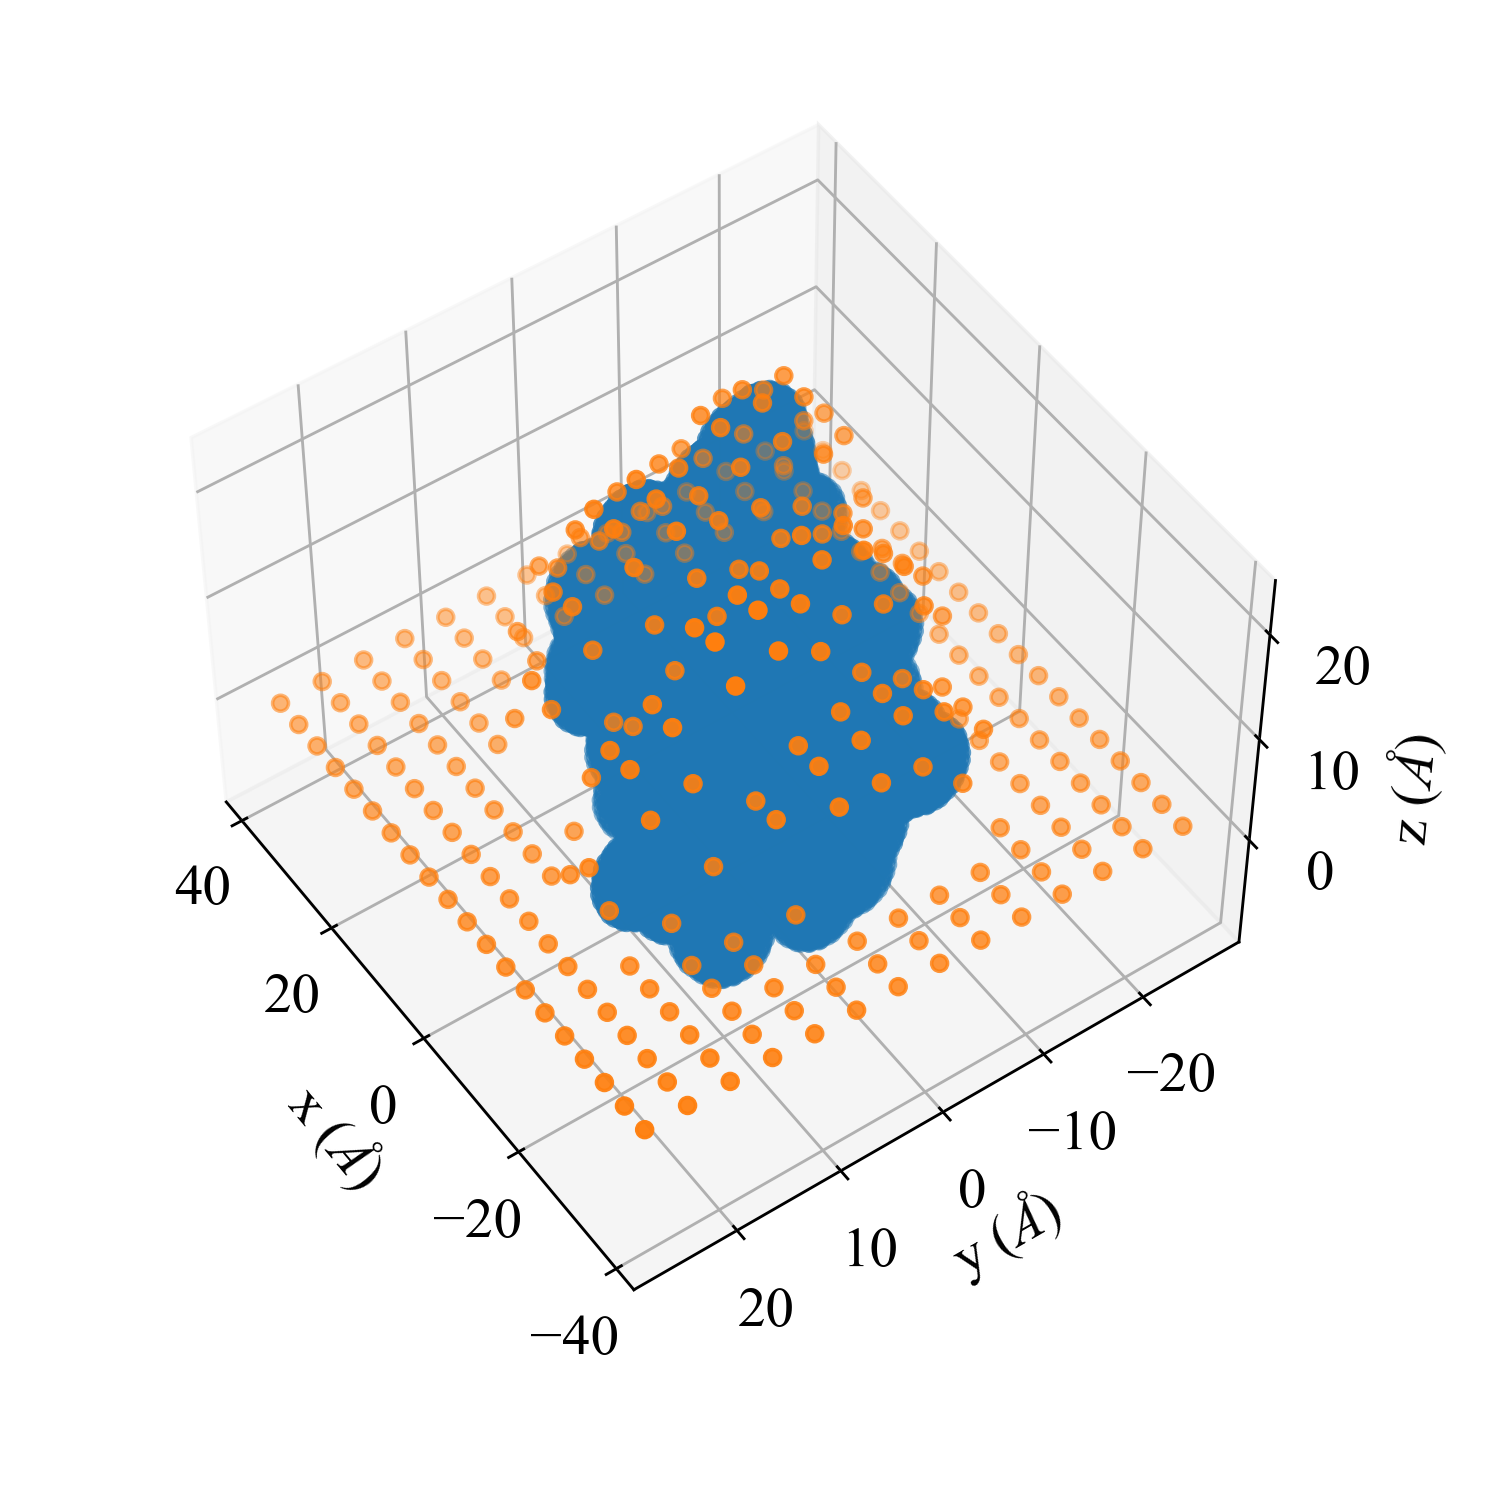
\includegraphics[width=1\linewidth]{Figures/AFMSimulationScanPos-1bna1.png} 
    \end{subfigure}
    \hfill
    \begin{subfigure}[t]{0.51\textwidth}
        \centering
        \caption{}
        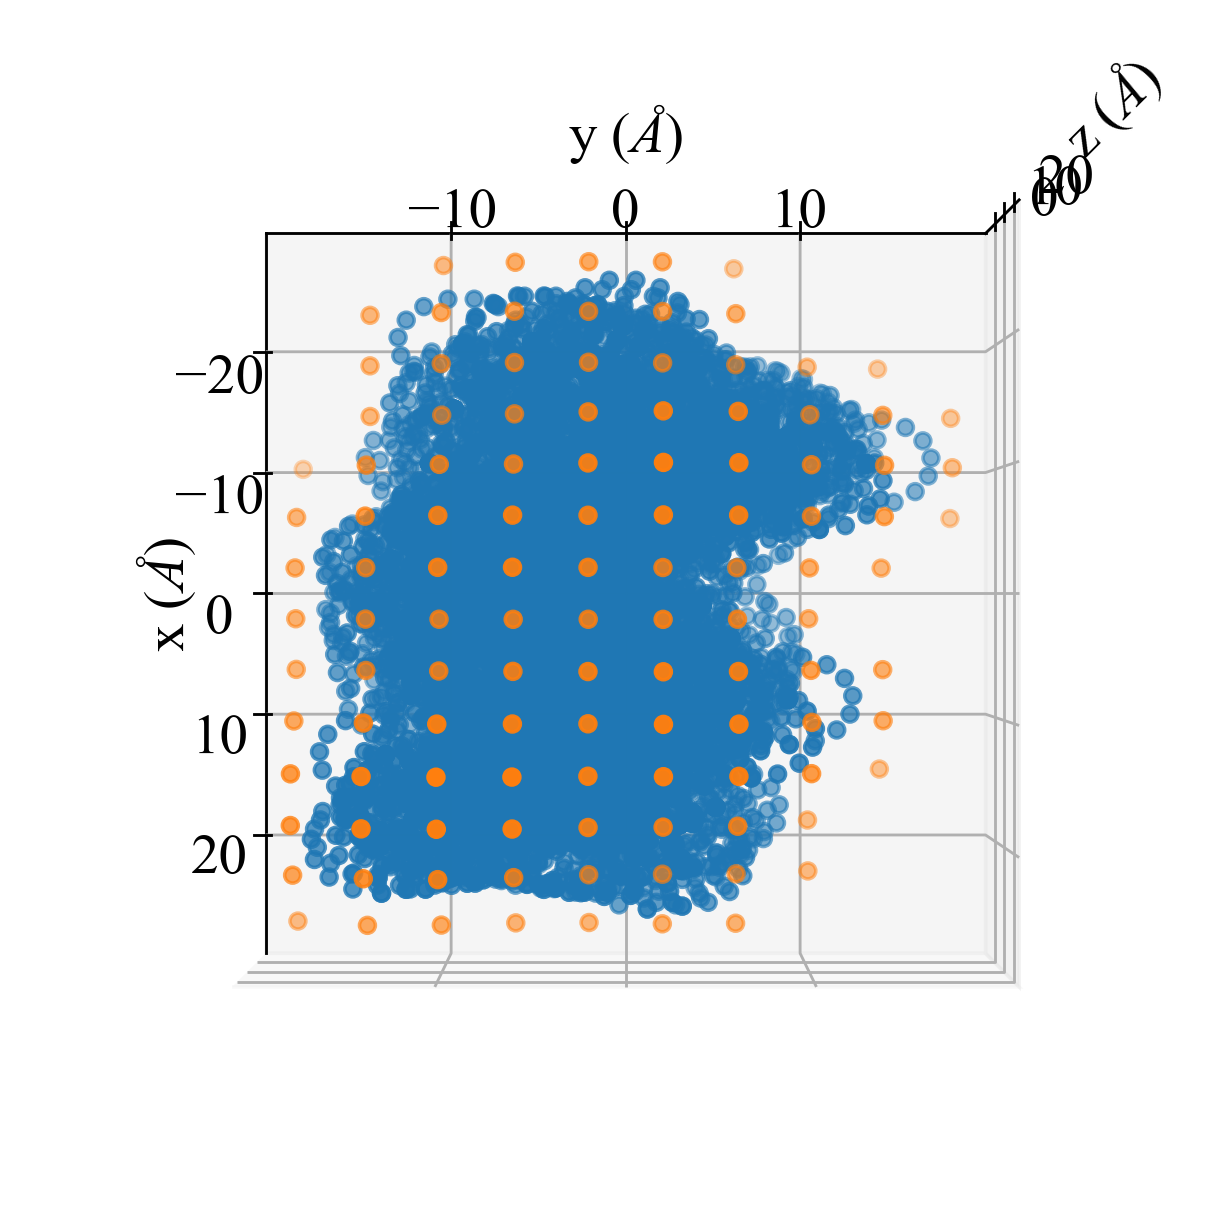
\includegraphics[width=1\linewidth]{Figures/AFMSimulationScanPos-1bna2.png}
    \end{subfigure} 
    
    \hfill
    \vspace{-0.4in}
    
    \begin{subfigure}[t]{0.49\textwidth}
        \centering
        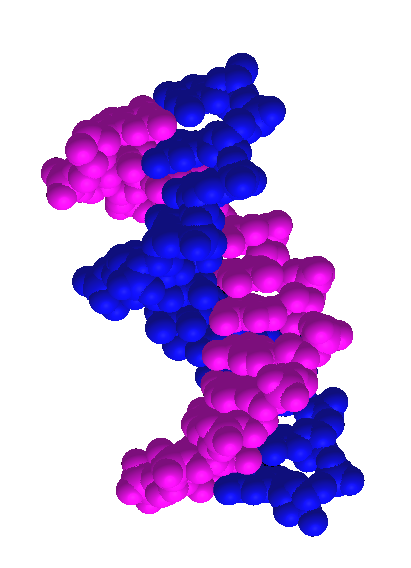
\includegraphics[width=0.35\linewidth, angle=10]{Figures/1BNA_veiw1.png}
    \end{subfigure} 
    \hfill
    \begin{subfigure}[t]{0.49\textwidth}
        \centering
        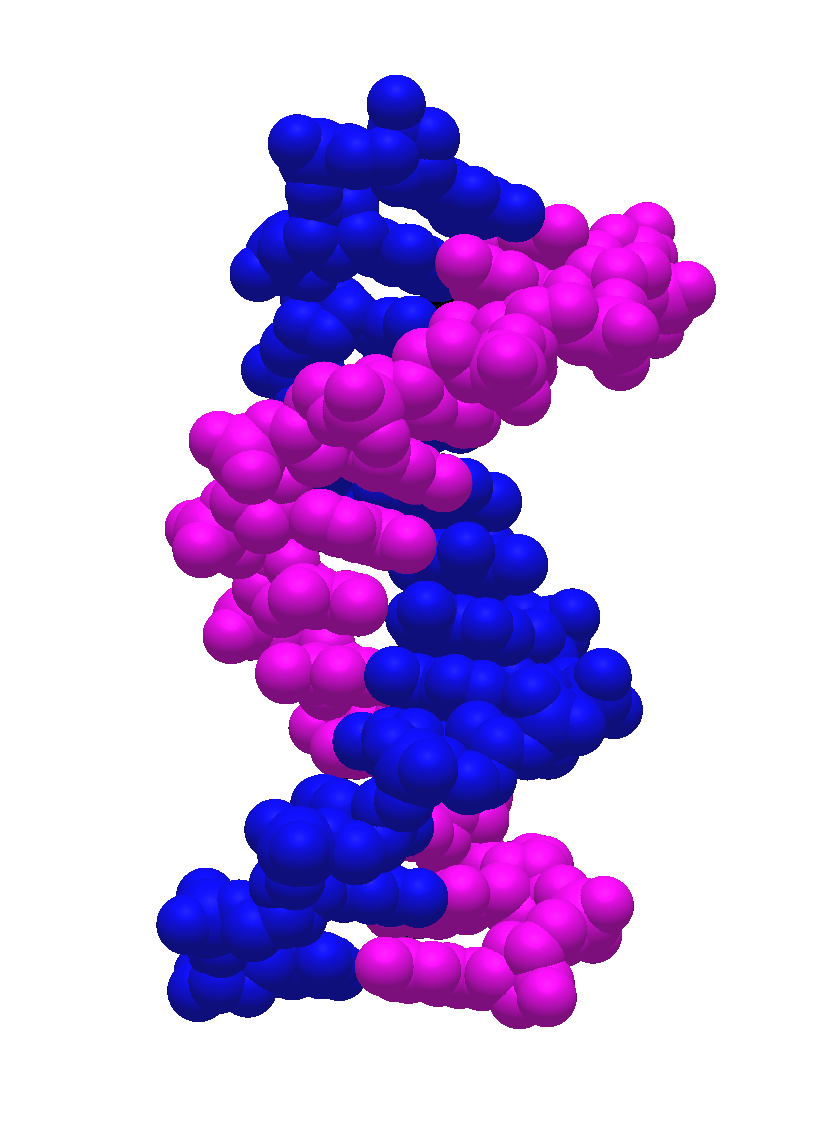
\includegraphics[width=0.35\linewidth]{Figures/1BNA_veiw2.png}
    \end{subfigure} 
    
    
    
    \caption{\label{fig: 1BNA Scan Position}Illustration of biomolecule (blue) and scan positions for simulation (orange). Sphere model of PDB below each to aid in visualisation. (A) Side view of the assembly with all scan positions. (B) Top view of the assembly with clipped scan points (only points where tip interacts) }
\end{figure}

As presented in Figure \ref{fig: 1BNA AFM Image}, our simulation has reproduced the expected appearance of the DNA double helix. This provides an example of the viability of the FEM approach to AFM imaging. We see distinct differences in the simulations produced with ABAQUS compared to the hard-sphere model in Figure \ref{fig: 1BNA AFM Image HS}. The indentation produces with FEM shows greater sensitivity for protruding features, whereas the deeper structure requires greater indentation/force to recover the surface topology. Similarly, simulating another orientation of the B-DNA, shown in Figure \ref{fig: 1BNA AFM Image-2}, revealed the utility of the FEM approach. The base for these simulations was divided into bins of 10 $\text{\AA}$ producing 38 individual scan positions/ ABAQUS simulations. The AFM probe tip was modelled with a radius of 10 $\text{\AA}$ and a conical half-angle $10^{o}$. The FEM simulation reproduced more underlying helix structure than the hard-sphere model. The hard sphere model for this simulation gave a blurred image of the DNA as the large tip distorts the surface. The surface indentation produced by FEM appears to recover elements of the underlying structure. However, some of these variations originate from ABAQUS not performing calculations at the points of complex deformation. Within the code, these points are set to the maximum indentation depth so appear artificially deeper. This could pose challenges in repeatability. 

\begin{figure}[H]
\centering
    \begin{subfigure}[t]{0.49\textwidth}
        \centering
        \caption{\label{fig: 1BNA AFM Image} }
        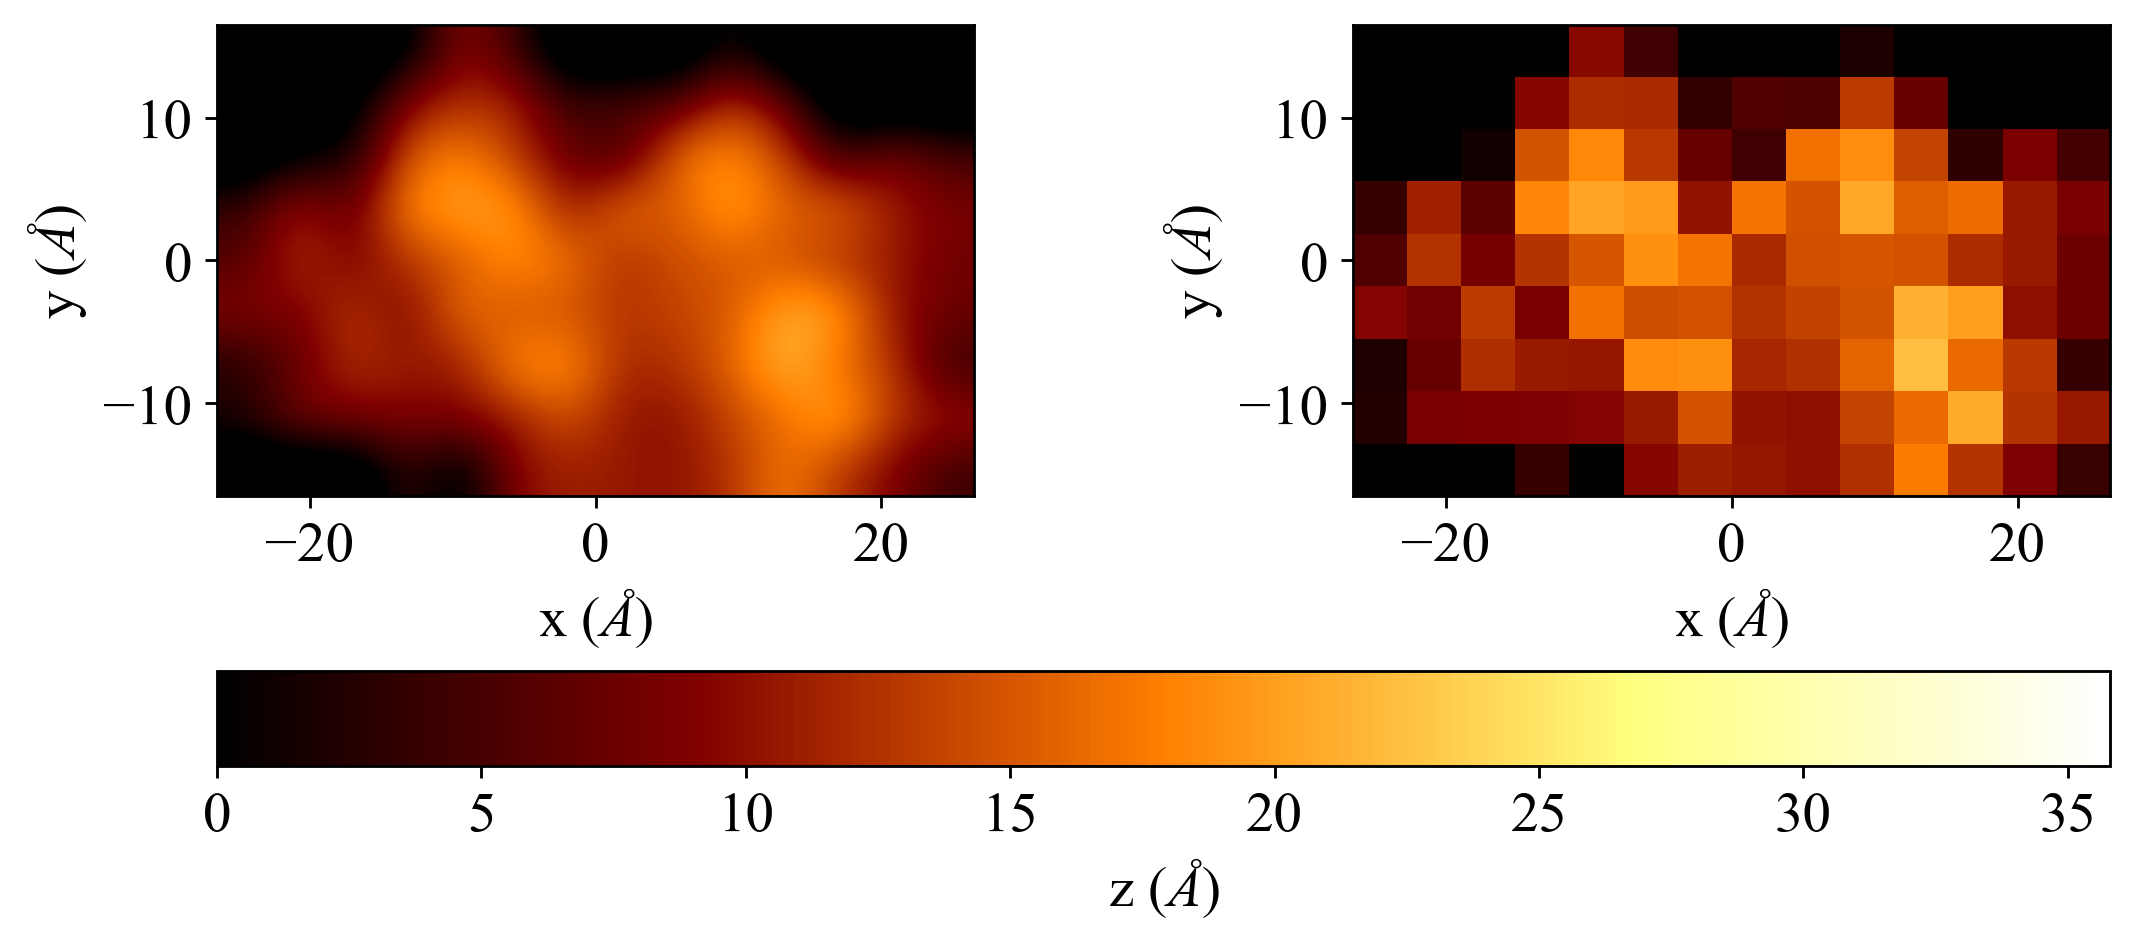
\includegraphics[width=1\linewidth]{Figures/AFMSimulationMolecule-1bna.png}
        
    \end{subfigure}
    \hfill
    \begin{subfigure}[t]{0.49\textwidth}
        \centering
        \caption{\label{fig: 1BNA AFM Image HS} }
        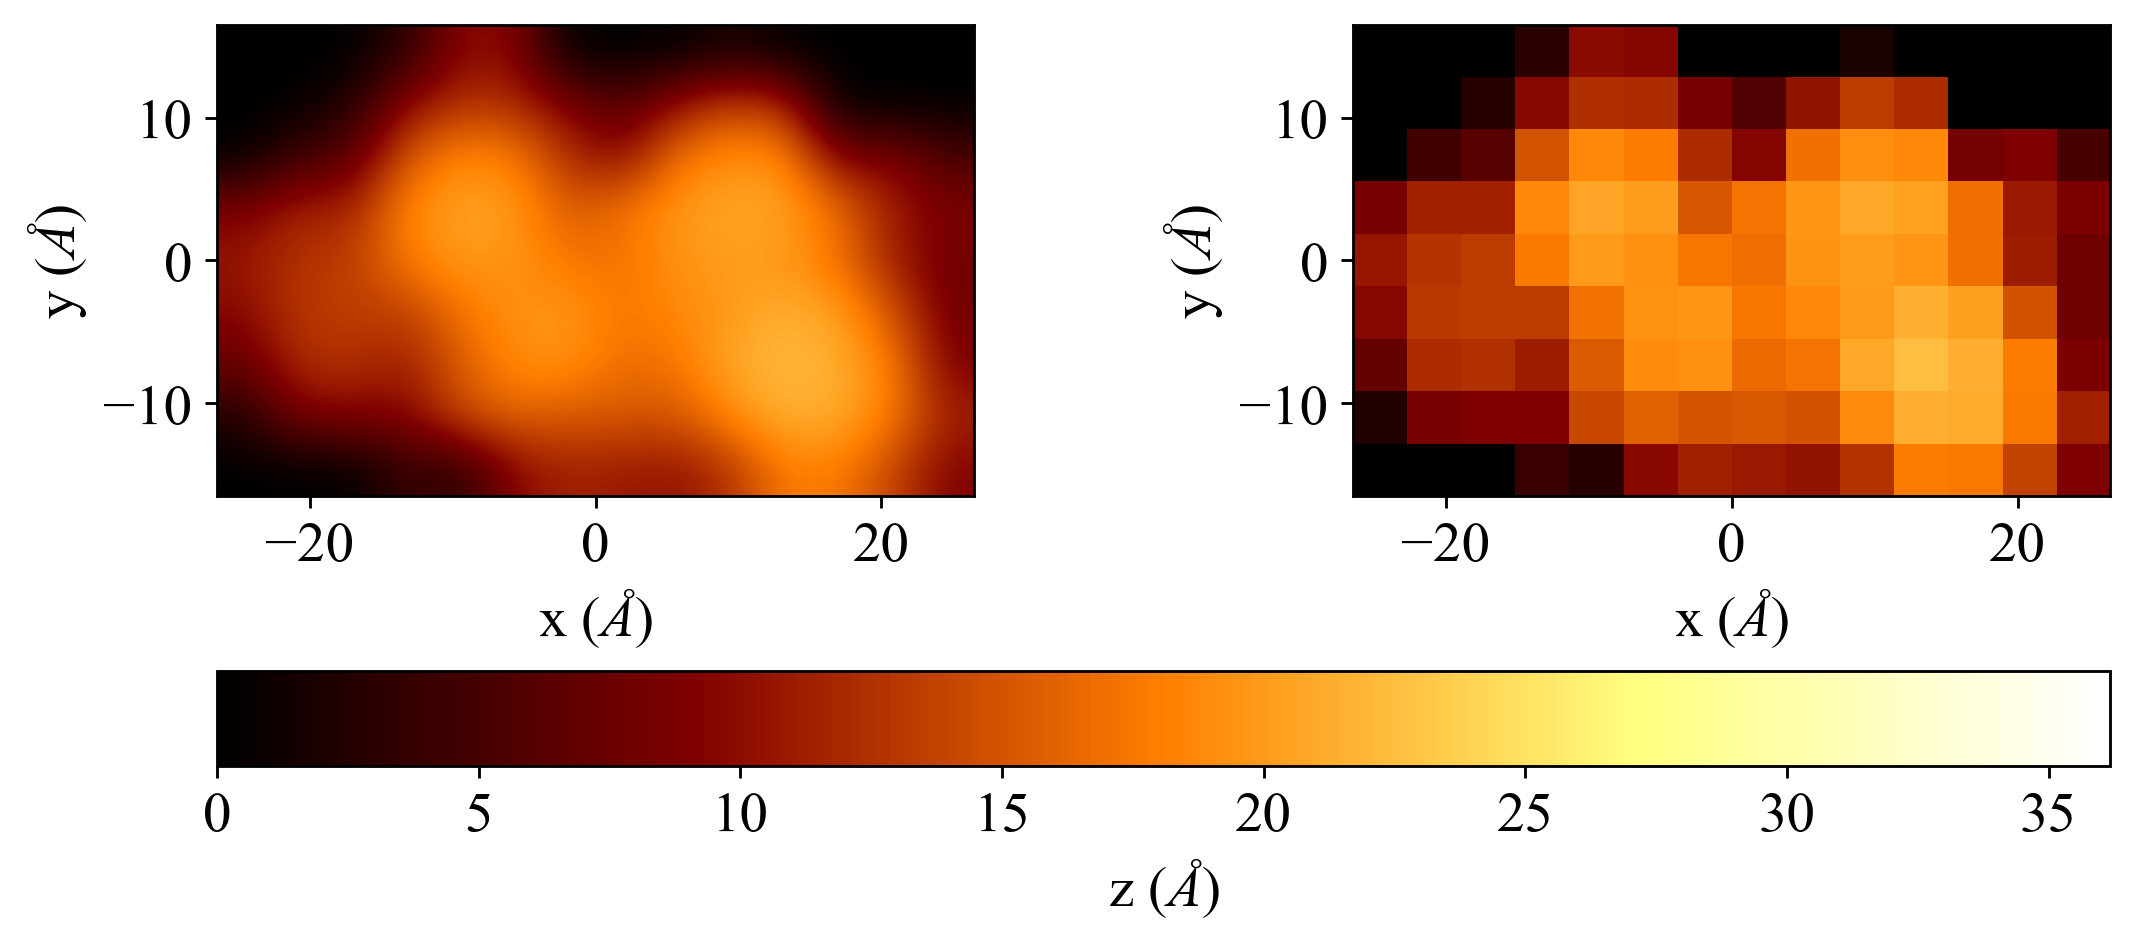
\includegraphics[width=1\linewidth]{Figures/AFMSimulationMolecule-1bna_HS.png}
    \end{subfigure}    

    \hfill
    
    \begin{subfigure}[t]{0.49\textwidth}
        \centering
        \caption{\label{fig: 1BNA AFM Image-2} }
        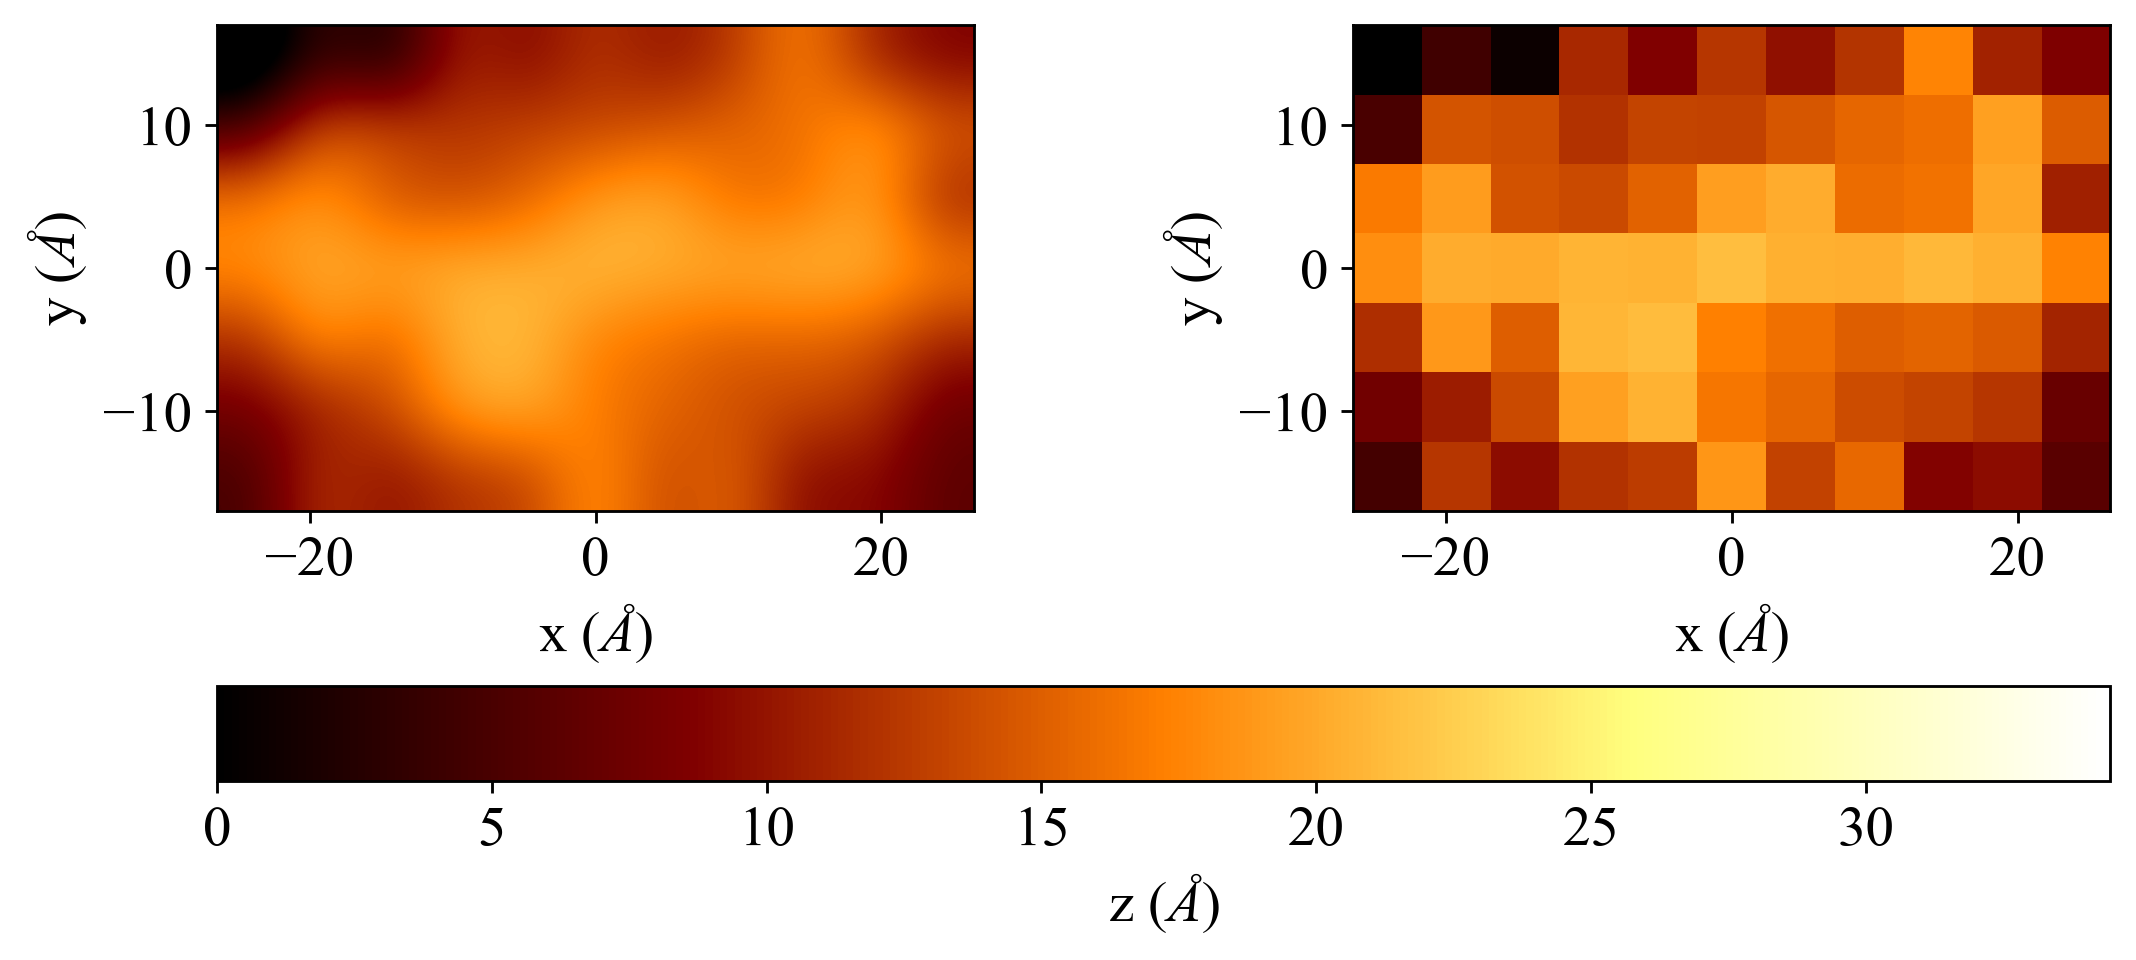
\includegraphics[width=1\linewidth]{Figures/AFMSimulationMolecule-1bna-2.png}
    \end{subfigure}
    \hfill
    \begin{subfigure}[t]{0.49\textwidth}
        \centering
        \caption{\label{fig: 1BNA AFM Image HS-2} }
        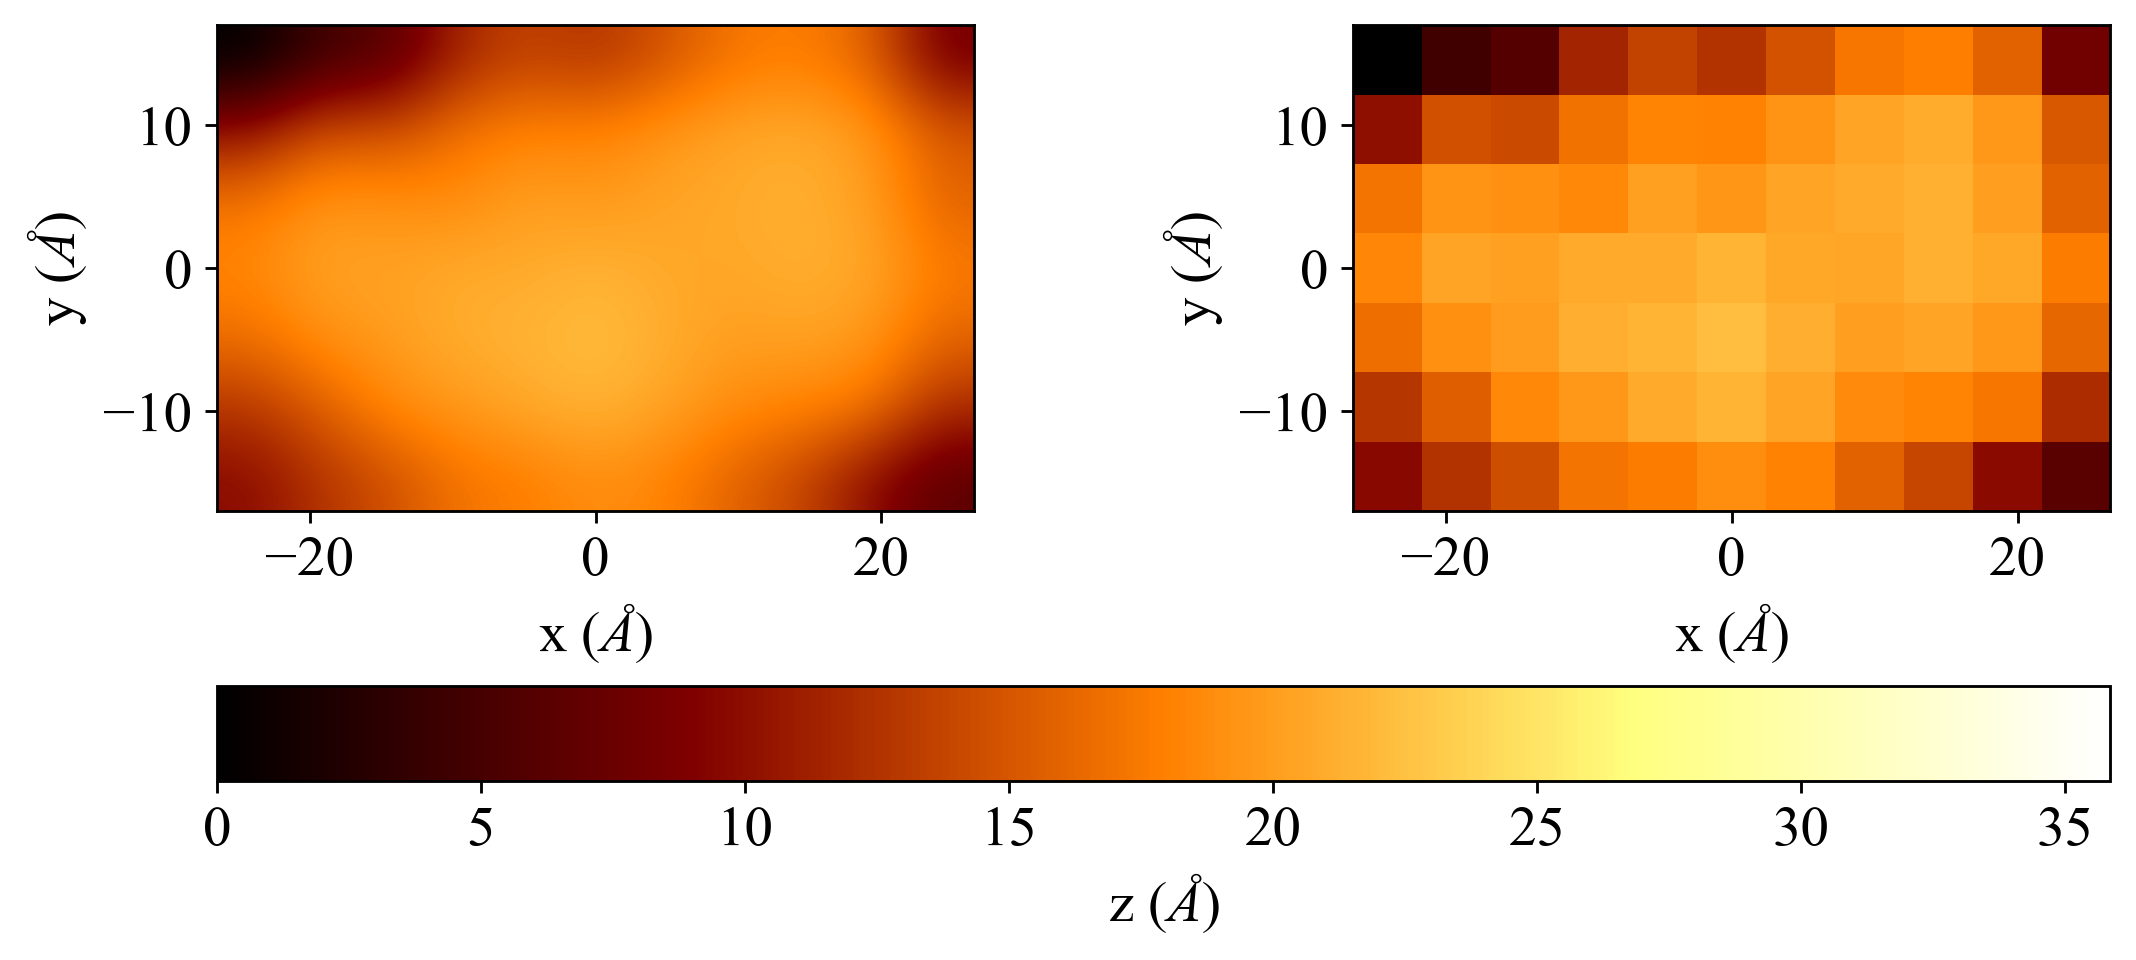
\includegraphics[width=1\linewidth]{Figures/AFMSimulationMolecule-1bna_HS-2.png}
    \end{subfigure}    
    
    \caption{\label{fig: 1BNA AFM}AFM images of a B-DNA DODECAMER with interpolated (left) and raw image(right) for each. (A) FEM Simulation with a tip radius of $4 \text{\AA}$ and spatial resolution of $4 \text{\AA}$ per pixel. (B) Hard sphere simulation with a tip radius of $4 \text{\AA}$ and spatial resolution of $4 \text{\AA}$ per pixel. (C) FEM simulation with a tip radius of $1 nm$ and spatial resolution of $1 nm$ per pixel.(D) Hard sphere simulation with a tip radius of $1 nm$ and spatial resolution of $1 nm$ per pixel.}
    
\end{figure}